\chapter{Signal conditioning system design}
\section{System overview} \label{sec:system}
%Here you insert a block diagram of your operational signal conditioning system. There is no need to specify the capacitor and resistor values here, but you want to capture the higher-level functional arrangement you have opted for. The diagram ties together the other chapters in this report and helps the reader understand how you have connected the different funtional blocks together to produce the outputs. For example, a block could be ``Differential aplifier'' or ``level shifting op-amps'' or the like. Fig.\ \ref{fig:system_diagram} as an example that is completely irrelevant and just holds space. 

A system capable of measuring voltages and currents as well as the phase differences between these sinusoids can be seen in Figure \ref{fig:system_diagram}. Load voltage levels were stepped down using a voltage divider before measurements, and the current through the load was measured by amplifying the voltage over the sense resistor. Phase differences were measured by using comparators and a XOR gate to generate a PWM signal, this PWM signal was then scaled to a voltage level by using a simple low pass filter. The TLC2222 op-amp was chosen for this design, and given that \SI{2.4}{mA} per op-amp could be expected \ref{yourmom}, only two op-amps utilized the \SI{-5}{V} regulator for their negative rail as to not compromise its integrity.

\begin{figure}
    \centering
    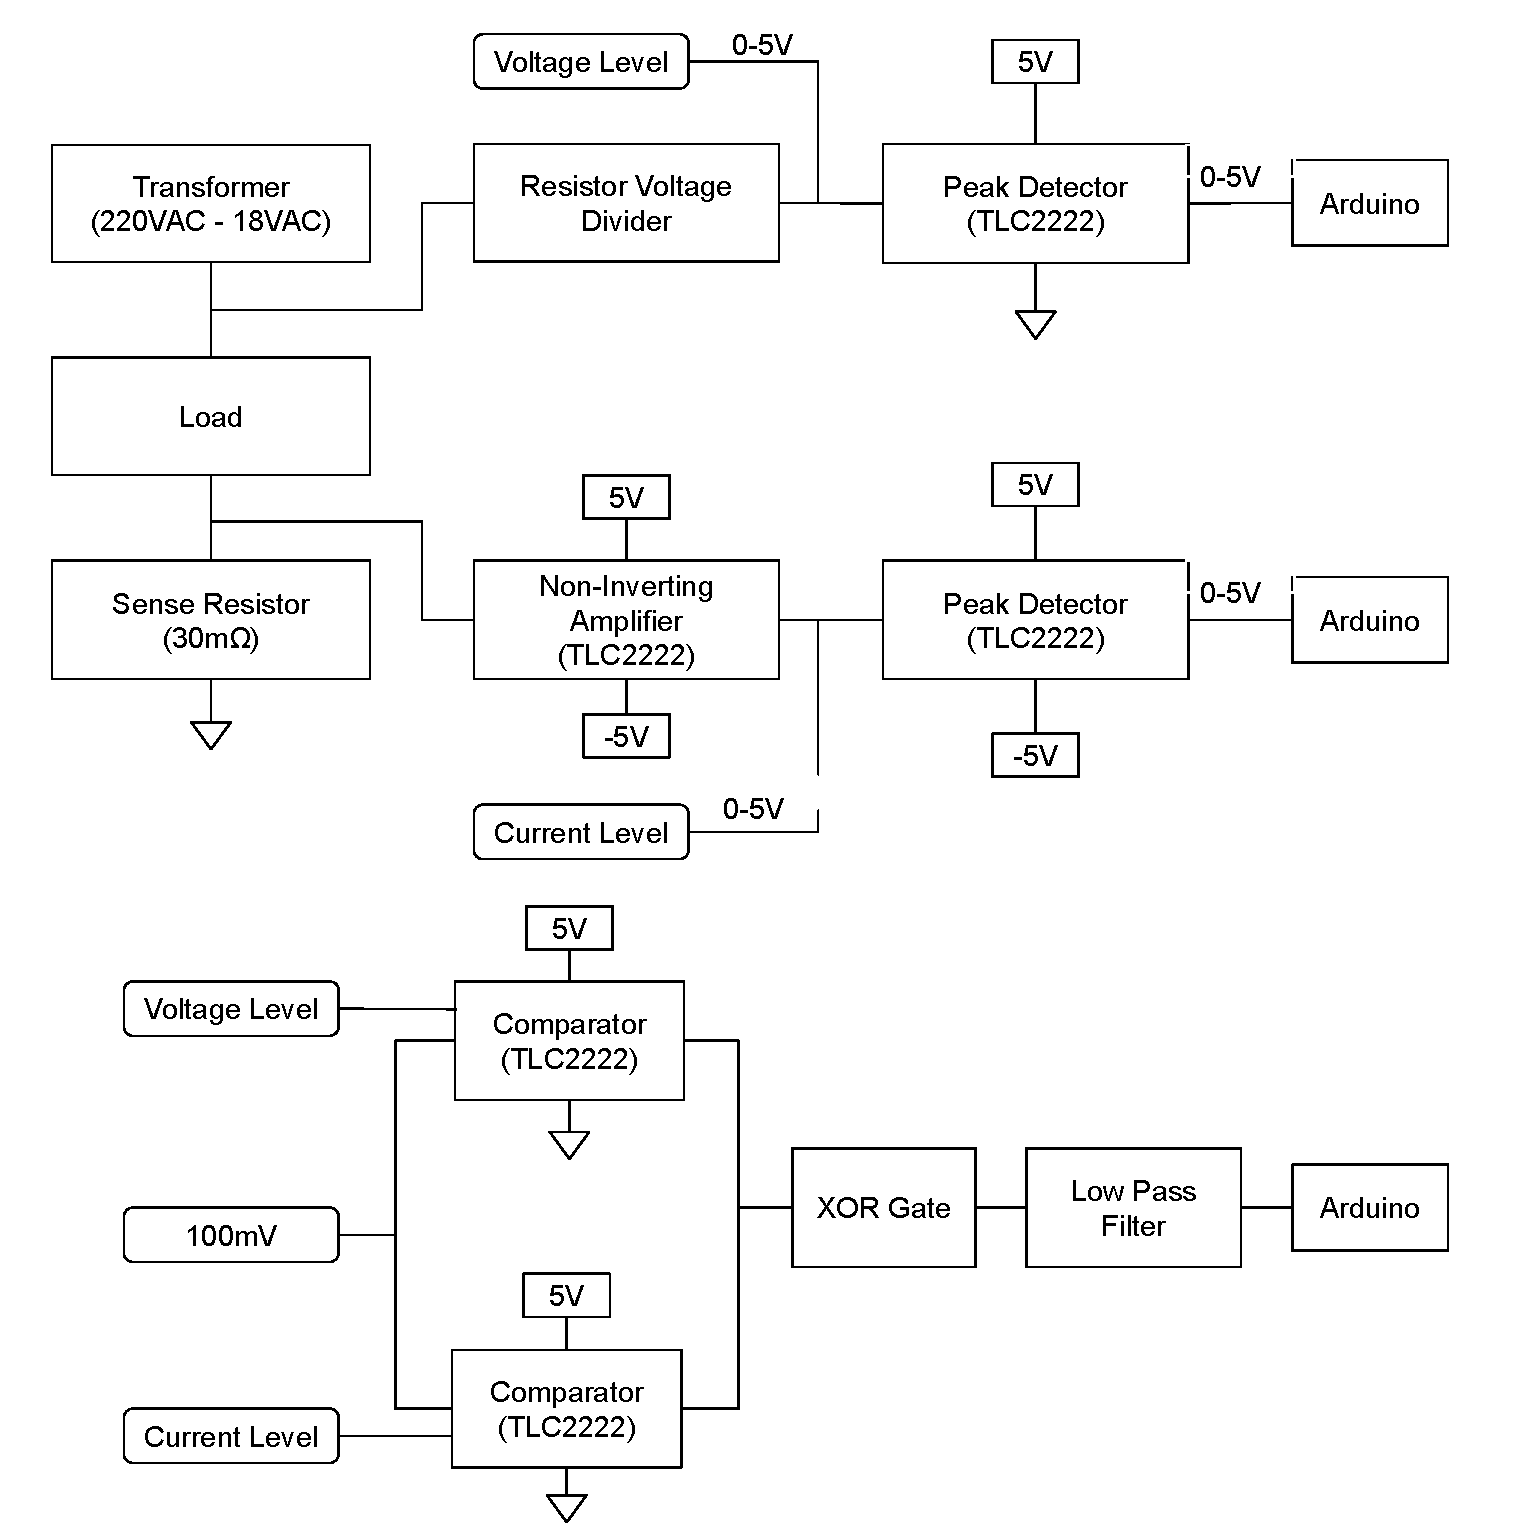
\includegraphics[width = 0.45\linewidth]{Figures/measurement_diagram.pdf}
    \caption{Signal Conditioning Diagram}
    \label{fig:system_diagram}
\end{figure}









